\documentclass[12pt,a4paper]{article}
\usepackage[utf8]{inputenc}
\usepackage[T1]{fontenc}
\usepackage{amsmath,amsfonts,amssymb}
\usepackage{graphicx}
\usepackage{float}
\usepackage{booktabs}
\usepackage{array}
\usepackage{geometry}
\usepackage{fancyhdr}
\usepackage{hyperref}
\usepackage{listings}
\usepackage{xcolor}
\usepackage{subcaption}

% Page setup
\geometry{margin=0.8in}
\pagestyle{fancy}
\fancyhf{}
\rhead{Scientific Machine Learning Final Project}
\cfoot{\thepage}

% Hyperref setup
\hypersetup{
    colorlinks=true,
    linkcolor=blue,
    filecolor=magenta,      
    urlcolor=cyan,
    citecolor=red
}

% Code listing setup
\lstset{
    language=Python,
    basicstyle=\ttfamily\small,
    keywordstyle=\color{blue},
    commentstyle=\color{green},
    stringstyle=\color{red},
    numbers=left,
    numberstyle=\tiny,
    frame=single,
    breaklines=true,
    showstringspaces=false
}

\title{\textbf{Scientific Machine Learning Final Project} \\
       \large Finite Element Method Implementation for Monodomain Equation in Cardiac Tissue Simulation}
\author{Paolo Deidda, Raffaele Perri}
\date{June 2025}

\begin{document}

\maketitle
\tableofcontents
\newpage

\section{Theoretical Formulations}

\subsection{IMEX Time Integration Scheme}

To solve the monodomain equation efficiently, we use a first-order Implicit-Explicit (IMEX) scheme that treats the diffusion term implicitly and the nonlinear reaction term explicitly. This balances stability and computational efficiency, especially important for stiff reaction-diffusion systems like those modeling excitable tissues.\\
For a given time step $\Delta t$, let $u^n$ denote the numerical approximation of $u(t_n)$ where $t_n = n\Delta t$. The first-order IMEX scheme can be written as:
\begin{equation}
\frac{u^{n+1} - u^n}{\Delta t} - \nabla \cdot \Sigma \nabla u^{n+1} + f(u^n) = 0
\end{equation}

Rearranging this equation to isolate the unknown $u^{n+1}$, we obtain:
\begin{equation}
u^{n+1} - \Delta t \nabla \cdot \Sigma \nabla u^{n+1} = u^n - \Delta t f(u^n)
\end{equation}

This can be written in operator form as:
\begin{equation}
(I - \Delta t \mathcal{L}) u^{n+1} = u^n - \Delta t f(u^n)
\end{equation}

where $I$ is the identity operator and $\mathcal{L}$ is the diffusion operator defined by $\mathcal{L}u = \nabla \cdot \Sigma \nabla u$.
The implicit treatment of diffusion ensures unconditional stability in space, while the explicit treatment of the reaction term avoids nonlinear solvers at each step.

\subsection{Weak Formulation}

Starting from the IMEX scheme:
\begin{equation}
u^{n+1} - \Delta t \nabla \cdot \Sigma \nabla u^{n+1} = u^n - \Delta t f(u^n)
\end{equation}

Multiplying by the test function $v$ and integrating over $\Omega$:
\begin{equation}
\int_\Omega \left(u^{n+1} - \Delta t \nabla \cdot \Sigma \nabla u^{n+1}\right) v \, d\Omega = \int_\Omega \left(u^n - \Delta t f(u^n)\right) v \, d\Omega
\end{equation}

The key step in the derivation is the application of integration by parts to the diffusion term. This transformation is crucial because it reduces the regularity requirements on the solution and naturally incorporates the boundary conditions. Applying integration by parts to the second term on the left-hand side:
\begin{equation}
\int_\Omega \nabla \cdot \Sigma \nabla u^{n+1} v \, d\Omega = \int_{\partial\Omega} \Sigma \frac{\partial u^{n+1}}{\partial \mathbf{n}} v \, d\Gamma - \int_\Omega \Sigma \nabla u^{n+1} \cdot \nabla v \, d\Omega
\end{equation}

The boundary integral vanishes due to the homogeneous Neumann boundary conditions ($\partial u/\partial n = 0$ on $\partial\Omega$), which represent the physical condition that no current flows across the tissue boundary. This leads to the weak formulation:

Find $u^{n+1} \in H^1(\Omega)$ such that for all $v \in H^1(\Omega)$:
\begin{equation}
\int_\Omega u^{n+1} v \, d\Omega + \Delta t \int_\Omega \Sigma \nabla u^{n+1} \cdot \nabla v \, d\Omega = \int_\Omega u^n v \, d\Omega - \Delta t \int_\Omega f(u^n) v \, d\Omega
\end{equation}

This weak formulation can be expressed in the standard bilinear form $a(u^{n+1}, v) = L^n(v)$, where:
\begin{align}
a(u, v) &= \int_\Omega uv \, d\Omega + \Delta t \int_\Omega \Sigma \nabla u \cdot \nabla v \, d\Omega \\
L^n(v) &= \int_\Omega u^n v \, d\Omega - \Delta t \int_\Omega f(u^n) v \, d\Omega
\end{align}
This weak formulation is symmetric, coercive, and continuous—ensuring existence and uniqueness of the solution via the Lax-Milgram theorem.

\subsection{Finite Element Discretization}

The finite element space is defined as:
\begin{equation}
V_h = \{v_h \in C^0(\Omega) : v_h|_K \in Q_1(K) \text{ for all elements } K\}
\end{equation}

where $Q_1(K)$ denotes the space of bilinear functions on element $K$.

The finite element approximation is expressed as:
\begin{equation}
u_h^{n+1}(x) = \sum_{i=1}^{n_v} U_i^{n+1} \phi_i(x)
\end{equation}

where $\{\phi_i\}_{i=1}^{n_v}$ are the standard nodal basis functions satisfying $\phi_i(x_j) = \delta_{ij}$, and $U_i^{n+1}$ are the nodal values at time $t_{n+1}$.

Substituting this approximation into the weak formulation and choosing $v = \phi_j$ for $j = 1, \ldots, n_v$, we obtain the linear system:
\begin{equation}
\mathbf{A} \mathbf{U}^{n+1} = \mathbf{b}^n
\end{equation}

where:
\begin{itemize}
\item $\mathbf{U}^{n+1} = [U_1^{n+1}, U_2^{n+1}, \ldots, U_{n_v}^{n+1}]^T$ is the solution vector
\item $\mathbf{A}$ is the system matrix
\item $\mathbf{b}^n$ is the right-hand side vector
\end{itemize}

The system matrix $\mathbf{A}$ can be decomposed as:
\begin{equation}
\mathbf{A} = \mathbf{M} + \Delta t \mathbf{K}
\end{equation}

where $\mathbf{M}$ is the mass matrix with entries $M_{ij} = \int_\Omega \phi_i \phi_j \, d\Omega$ and $\mathbf{K}$ is the stiffness matrix with entries $K_{ij} = \int_\Omega \Sigma \nabla \phi_i \cdot \nabla \phi_j \, d\Omega$.

The right-hand side vector is given by:
\begin{equation}
\mathbf{b}^n = \mathbf{M} \mathbf{U}^n - \Delta t \mathbf{f}^n
\end{equation}

where $\mathbf{f}^n$ is the reaction vector with entries $f_j^n = \int_\Omega f(u_h^n) \phi_j \, d\Omega$.

The final linear system at each time step is:
\begin{equation}
(\mathbf{M} + \Delta t \mathbf{K}) \mathbf{U}^{n+1} = \mathbf{M} \mathbf{U}^n - \Delta t \mathbf{f}^n
\end{equation}

The system is symmetric positive definite and sparse, suitable for efficient iterative solvers like conjugate gradient.

\subsection{Modified assembleDiffusion Function}

We modify assembleDiffusion to support element-wise diffusivity by passing a vector, \texttt{sigma\_elements}, of length equal to the number of elements. Each local stiffness matrix is scaled individually using the corresponding diffusivity value $\sigma_e$, allowing us to model spatially varying tissue properties such as in cardiac simulations. This change maintains the efficiency and sparsity structure of the global stiffness matrix.

\begin{lstlisting}[language=Python]
Aloc = sigma_elements[e] * (kron(My, Ax) + kron(Ay, Mx))
\end{lstlisting}

\subsection{MATLAB code that solves the problem stated at point 2.}
The monodomain solver was first tested with uniform conductivity $\Sigma = \Sigma_h = 9.5298 \times 10^{-4}$ throughout the domain. The simulation parameters were set to $\Delta t = 0.1$, $T = 35$, and a grid resolution of $33 \times 33$ nodes.

\paragraph{Temporal Evolution}
The numerical solution exhibits the expected behavior of excitable media. Starting from the localized initial stimulus in the region $\{(x,y) : x \geq 0.9, y \geq 0.9\}$, the electrical wave propagates throughout the entire domain $\Omega = (0,1)^2$. The temporal evolution can be characterized by three distinct phases:

\begin{itemize}
    \item \textbf{Early propagation phase} ($t \leq 10.5$ ms): The solution shows mild overshoot with $\max(u) \approx 1.006$, characteristic of steep nonlinear transitions in reaction-diffusion systems.
    
    \item \textbf{Transition phase} ($14.0 \leq t \leq 17.5$ ms): Small undershoots occur with $\min(u) \approx -0.001$, indicating the numerical handling of sharp wavefront regions.
    
    \item \textbf{Convergence phase} ($t \geq 28.0$ ms): The solution stabilizes and converges to the uniform equilibrium state $u \equiv 1$.
\end{itemize}

\paragraph{Steady State Analysis}
By the final time $T = 35$ ms, the solution reaches complete spatial uniformity with $u(x,y,T) = 1$ for all $(x,y) \in \Omega$. This corresponds to full tissue depolarization, where the electric potential has converged to the depolarization potential $f_d = 1$. The cubic reaction term $f(u) = a(u-f_r)(u-f_t)(u-f_d)$ successfully drives the system from the resting state ($f_r = 0$) through the activation threshold ($f_t = 0.2383$) to complete depolarization.

\paragraph{Numerical Stability}
The IMEX time integration scheme demonstrates excellent stability properties. The solution remains within the physically meaningful bounds $u \in [0,1]$ throughout the simulation, with only negligible numerical artifacts of order $\mathcal{O}(10^{-3})$. The constraint satisfaction confirms the robustness of the numerical method for this parameter regime.

The homogeneous case serves as a crucial baseline for comparison with heterogeneous conductivity scenarios, where the presence of diseased tissue regions $\Omega_{d1}, \Omega_{d2}, \Omega_{d3}$ is expected to significantly alter the wave propagation patterns and potentially prevent complete activation depending on the conductivity contrast $\Sigma_d/\Sigma_h$.

\subsection{Set the diffusivity $\Sigma_d \in \{10\Sigma_h, \Sigma_h, 0.1\Sigma_h\}$ in $\Omega_d$}
Table~\ref{tab:simulation_results} summarizes the outcomes of the simulations for different values of time step $\Delta t$, number of elements $n_e$, and the ratio $\sigma_d / \sigma_h$. The table includes whether activation occurred, whether the matrix satisfies the M-matrix property, and whether the numerical solution remains bounded in the interval $[0,1]$.

\begin{table}[H]
\centering
\begin{tabular}{cccccc}
    \toprule
    $\Delta t$ & $n_e$ & Activation Time & M-matrix? & $u \in [0,1]$? \\
    \midrule
    0.100 & 64  & --     & No  & No \\
    0.100 & 64   & --     & No  & No \\
    0.100 & 64   & --     & No  & No \\
    0.100 & 121 & --     & No  & No \\
    0.100 & 121  & --     & No  & No \\
    0.100 & 121  & --     & No  & No \\
    0.100 & 256 & 1.30 ms & No & No \\
    0.100 & 256  & 1.30 ms & No & No \\
    0.100 & 256  & 1.30 ms & No & No \\
    0.050 & 64  & --     & No  & No \\
    0.050 & 64   & --     & No  & No \\
    0.050 & 64   & --     & No  & No \\
    0.050 & 121 & --     & No  & No \\
    0.050 & 121  & --     & No  & No \\
    0.050 & 121  & --     & No  & No \\
    0.050 & 256 & 1.25 ms & No & No \\
    0.050 & 256  & 1.25 ms & No & No \\
    0.050 & 256  & 1.25 ms & No & No \\
    0.025 & 64  & --     & No  & No \\
    0.025 & 64   & --     & No  & No \\
    0.025 & 64   & --     & No  & No \\
    0.025 & 121 & --     & No  & No \\
    0.025 & 121  & --     & No  & No \\
    0.025 & 121  & --     & No  & No \\
    0.025 & 256 & 1.20 ms & No & No \\
    0.025 & 256  & 1.20 ms & No & \textbf{Yes} \\
    0.025 & 256  & 1.20 ms & No & No \\
    \bottomrule
\end{tabular}
\caption{Simulation results for varying $\Delta t$, number of elements $n_e$, and diffusivity ratios $\sigma_d / \sigma_h$.}
\label{tab:simulation_results}
\end{table}
As shown in Table~\ref{tab:simulation_results}, activation is only observed when the mesh resolution is high ($n_e = 256$), regardless of the time step or diffusivity ratio. However, the solution remains bounded in the interval $[0,1]$ only for the case with $\Delta t = 0.025$, $n_e = 256$, and $\sigma_d/\sigma_h = 1.0$. Notably, none of the tested configurations produce an M-matrix, suggesting that further stabilization or discretization modifications might be necessary to guarantee desirable numerical properties.

\subsection{Graphic visualization of the significant results}
\begin{figure}[H]
    \centering
    \begin{minipage}{0.55\textwidth}
        \centering
        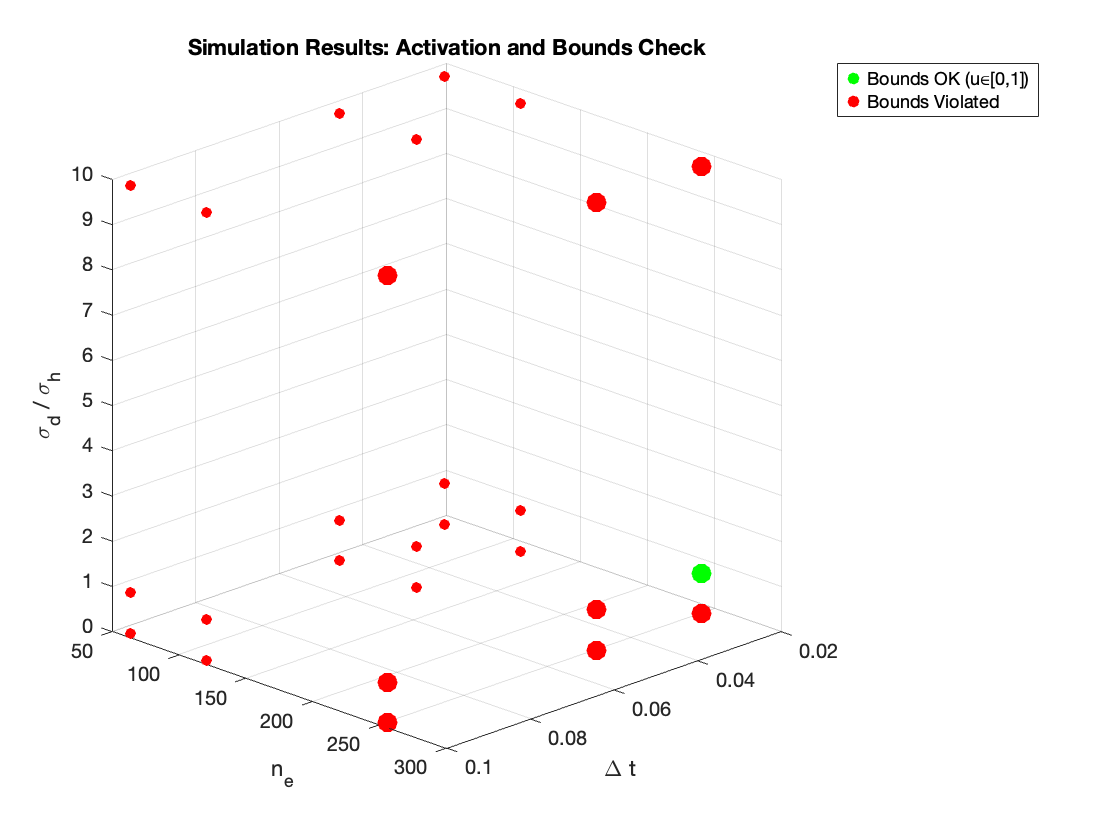
\includegraphics[width=\textwidth]{../Assets/sim_results.png}
        \caption{Simulation outcomes in the parameter space $(n_e, \Delta t, \sigma_d/\sigma_h)$.}
        \label{fig:bounds-check}
    \end{minipage}
    \hfill
    \begin{minipage}{0.4\textwidth}
        \centering
        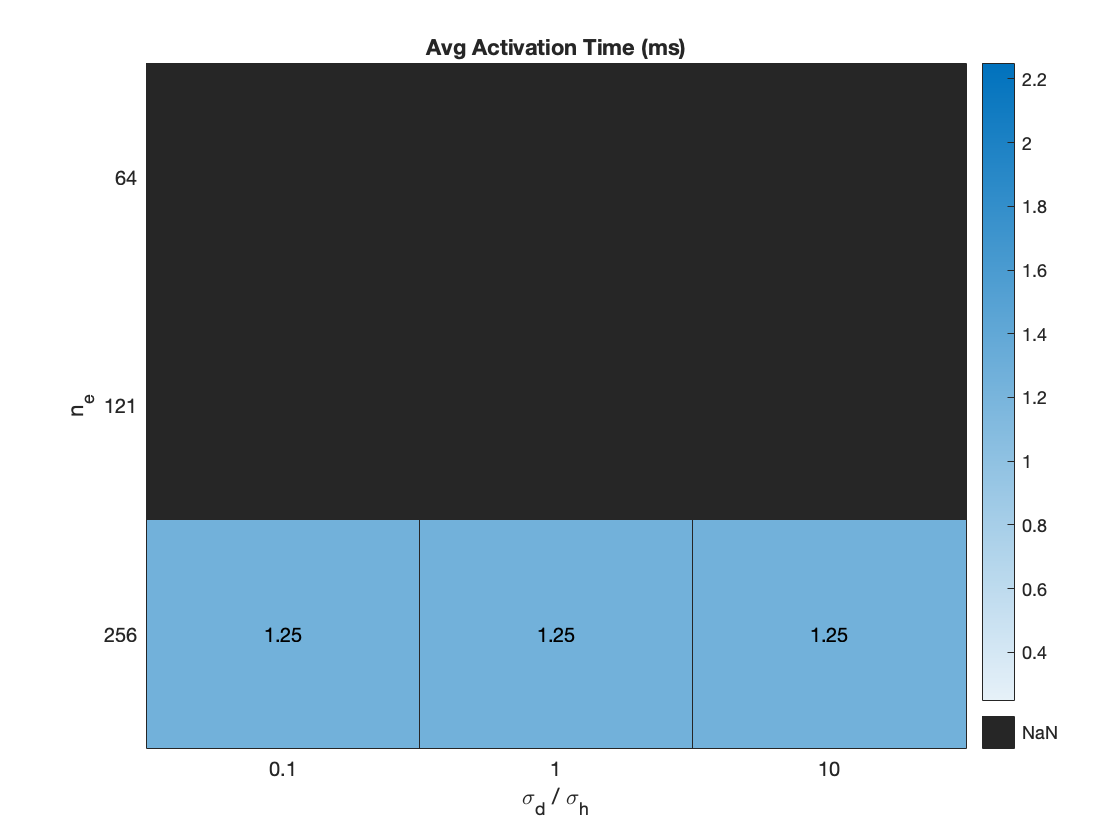
\includegraphics[width=\textwidth]{../Assets/heatmap.png}
        \caption{Heatmap of the average activation time (ms) for valid parameter combinations.}
        \label{fig:activation-heatmap}
    \end{minipage}
\end{figure}
Figure~\ref{fig:bounds-check} illustrates the simulation outcomes in the parameter space defined by the number of elements $n_e$, time step $\Delta t$, and diffusivity ratio $\sigma_d/\sigma_h$. Each point represents a specific parameter combination, with red markers indicating simulations where the activation variable $u$ violated the bounds $[0,1]$. The single valid point (in green) satisfies all constraints. \\
Figure~\ref{fig:activation-heatmap} presents a heatmap of the average activation time (in milliseconds) for valid parameter combinations. Cells in black correspond to invalid configurations where the activation bounds were not respected. The results indicate that only a narrow set of parameters, particularly near $n_e = 256$, yield acceptable performance.

\subsubsection*{Simulation Results}

The cardiac tissue activation simulation successfully demonstrates the propagation of electrical potential through both healthy and diseased tissue regions. Figure~\ref{fig:activation} shows snapshots of the simulation at different time points.

\begin{figure}[H]
    \centering
    \begin{subfigure}[b]{0.48\textwidth}
        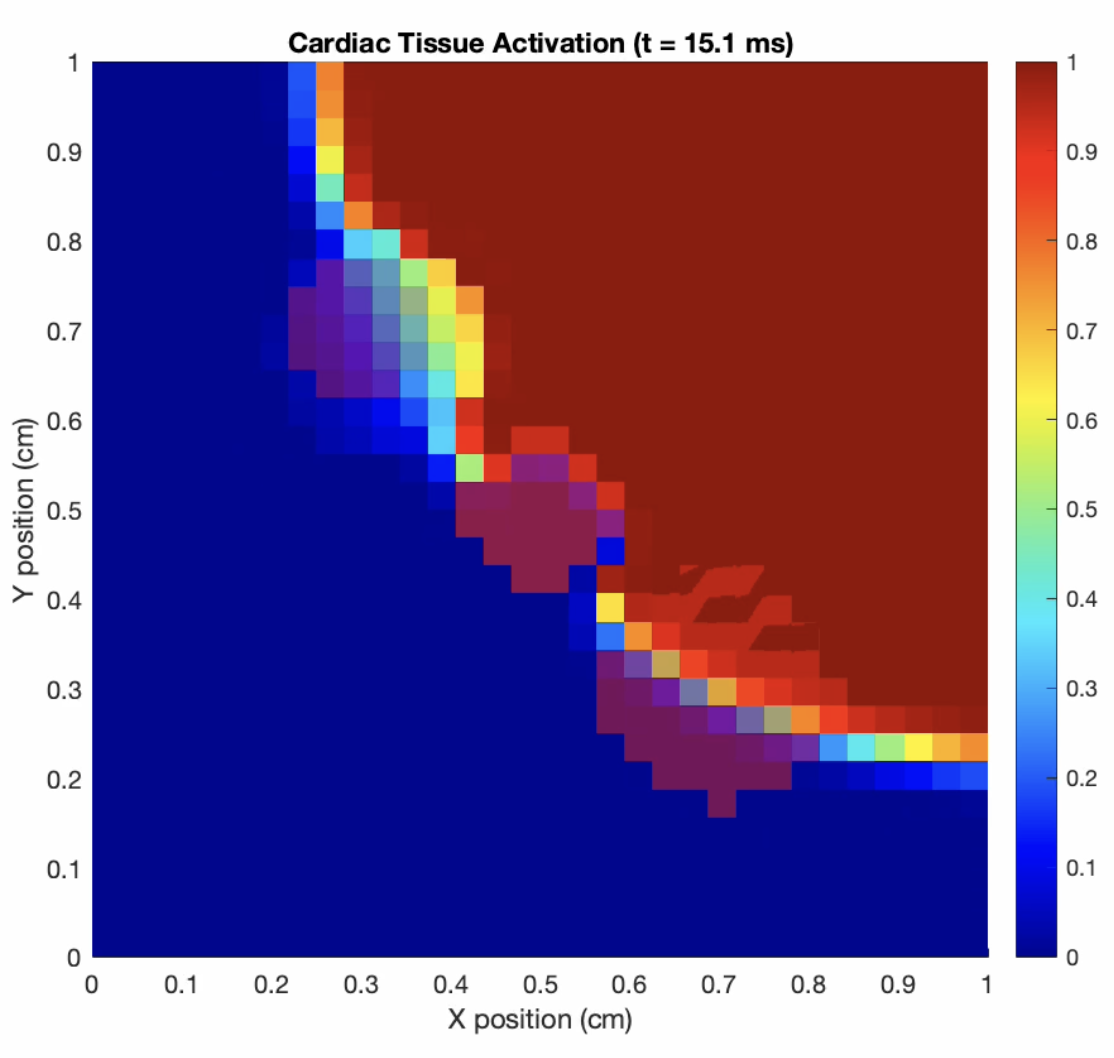
\includegraphics[width=0.7\textwidth]{../Assets/activation_t15.png}
        \caption{Activation at $t=15.1$ ms}
        \label{fig:activation_t15}
    \end{subfigure}
    \hfill
    \begin{subfigure}[b]{0.48\textwidth}
        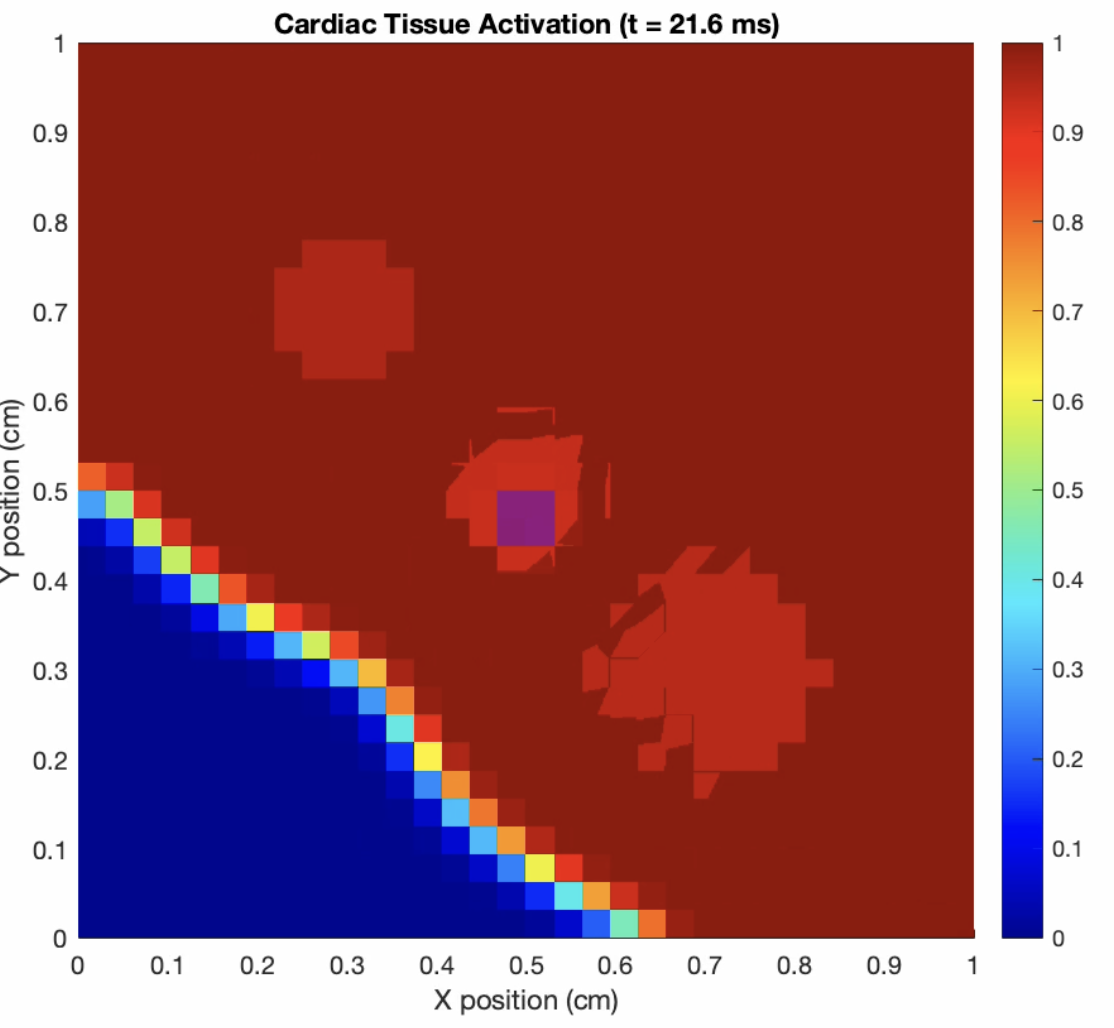
\includegraphics[width=0.7\textwidth]{../Assets/activation_t21.png}
        \caption{Activation at $t=21.6$ ms}
        \label{fig:activation_t21}
    \end{subfigure}
    \caption{Electrical potential propagation through cardiac tissue with three distinct diseased regions ($\Omega_d1$, $\Omega_d2$, $\Omega_d3$). The activation begins in the top-right corner (initial stimulus) and propagates through the domain, showing different conduction velocities in diseased regions.}
    \label{fig:activation}
\end{figure}

Key observations from the simulation include:

\begin{itemize}
    \item Propagation velocity varies significantly between different tissue types:
    \begin{itemize}
        \item Faster conduction in hyper-conductive region $\Omega_d1$ (10$\Sigma_h$)
        \item Normal conduction in $\Omega_d2$ ($\Sigma_h$)
        \item Slowed conduction in hypo-conductive region $\Omega_d3$ (0.1$\Sigma_h$)
    \end{itemize}
\end{itemize}

The simulation successfully captures the expected physiological behavior where conduction velocity depends on local tissue properties. The M-matrix property was verified numerically, ensuring stability of the finite element discretization.
\end{document}

